% 41039 Programming 1 revision; shared style copied from the established Week 4 deck.
\documentclass[aspectratio=169]{beamer}
\makeatletter

\usepackage{lmodern}
\usepackage{booktabs}
\usepackage{array}
\usepackage{graphicx}
\usepackage{xcolor}
\usepackage{listings}
\usepackage{pifont}
\usepackage{enumitem}
\usepackage[most]{tcolorbox}
\usepackage{tikz}
\usetikzlibrary{shapes.geometric, arrows.meta, positioning}

% Beamer's default enumerate label expands to itself once enumitem takes the optional
% argument, and TeX runs out of input stack. An explicit label breaks the loop.
\setlist[enumerate]{label=\arabic*.}
\setlist[itemize]{label=\usebeamertemplate{itemize item}}

\definecolor{bkblue}{RGB}{0,70,140}
\definecolor{bktitlebg}{RGB}{64,116,169}
\definecolor{codebg}{RGB}{244,246,249}
\definecolor{codecmt}{RGB}{110,120,130}
\definecolor{codegray}{RGB}{110,120,135}
\definecolor{codestr}{RGB}{150,60,20}
\definecolor{badred}{RGB}{185,40,40}
\definecolor{goodgreen}{RGB}{20,125,70}
\definecolor{srcgrey}{RGB}{105,115,128}

\usetheme{default}
\useinnertheme{rounded}
\setbeamertemplate{navigation symbols}{}

\setbeamercolor{titlelike}{bg=bktitlebg,fg=white}
\setbeamercolor{frametitle}{fg=bkblue,bg=}
\setbeamercolor{author}{fg=bkblue}
\setbeamercolor{institute}{fg=bkblue}
\setbeamercolor{section in toc}{fg=bkblue}
\setbeamerfont{frametitle}{size=\Large,series=\mdseries}
\setbeamerfont{title}{size=\Large,series=\bfseries}
\setbeamerfont{subtitle}{size=\normalsize,series=\bfseries}

\setbeamertemplate{frametitle}{%
  \vspace*{0.35em}%
  \begin{minipage}[b]{0.84\textwidth}%
    \usebeamerfont{frametitle}\usebeamercolor[fg]{frametitle}\insertframetitle%
  \end{minipage}\hfill%
  \begin{minipage}[b]{0.10\textwidth}%
    \raggedleft
\includegraphics[height=0.75cm]{bk-logo.png}%
  \end{minipage}\\[0.1em]%
  {\color{bkblue}\rule{\textwidth}{0.7pt}}%
}

\setbeamercolor{footbar}{bg=bkblue,fg=white}
\setbeamertemplate{footline}{%
  \begin{beamercolorbox}[wd=\paperwidth,ht=2.1ex,dp=1.1ex,leftskip=.3cm,rightskip=.3cm]{footbar}%
    \tiny\insertshorttitle\hfill\insertframenumber{}/\inserttotalframenumber%
  \end{beamercolorbox}%
}

\newcommand{\keyline}[1]{\vfill\begin{center}\textcolor{bkblue}{\textbf{#1}}\end{center}\vspace*{0.2em}}
\newcommand{\hd}[1]{\textbf{#1}}
\newcommand{\code}[1]{\texttt{#1}}
\newcommand{\srcline}[1]{{\color{srcgrey}\scriptsize #1\par}}
\newcommand{\srclink}[2]{\href{#1}{\texttt{#2}}}
\newcommand{\badlabel}[1]{\textcolor{badred}{\ding{55}~\textbf{#1}}}
\newcommand{\goodlabel}[1]{\textcolor{goodgreen}{\ding{51}~\textbf{#1}}}
\newcommand{\neutrallabel}[1]{\textcolor{bkblue}{\textbf{#1}}}
\newcommand{\timing}[2]{\hfill{\small\textcolor{bkblue}{\textbf{#1 \textbullet{} #2}}}}
% a blank to be filled in, numbered so the word bank can be checked against it
\newcommand{\blank}[1]{\underline{\hspace{1.1em}\textbf{(#1)}\hspace{1.1em}}}
\newcommand{\yes}{\textcolor{goodgreen}{\ding{51}}}
\newcommand{\no}{\textcolor{badred}{\ding{55}}}

% --- Stack and heap pictures (Draw it) --------------------------------------
\tikzset{
  sframe/.style={draw=bkblue, thick, fill=codebg, rounded corners=2pt, inner sep=4pt,
    font=\scriptsize\ttfamily, align=left, anchor=north west},
  ftitle/.style={font=\scriptsize\sffamily\bfseries, text=bkblue, anchor=south west},
  cell/.style={draw=bkblue, fill=white, font=\scriptsize\ttfamily, minimum width=0.62cm,
    minimum height=0.5cm, inner sep=1pt},
  atitle/.style={font=\scriptsize\ttfamily, text=bkblue, anchor=south west, inner sep=1pt},
  ref/.style={-{Stealth[length=5pt]}, thick, draw=bkblue!85!black},
  hd/.style={font=\small\sffamily\bfseries, text=bkblue},
}

\hypersetup{colorlinks=true, urlcolor=bkblue, linkcolor=bkblue}

% --- Question box: what the room is being asked --------------------------
\newtcolorbox{discussionbox}[1]{
  title=\textbf{#1}, coltitle=bkblue, colback=white, colframe=bkblue,
  colbacktitle=bkblue!10, boxrule=1pt, arc=3pt,
  left=6pt, right=6pt, top=4pt, bottom=4pt
}
% --- Answer box: revealed after they have committed to an answer ---------
\newtcolorbox{contextbox}[1]{
  title=\textbf{#1}, coltitle=white, colback=bkblue!5, colframe=bkblue,
  colbacktitle=bkblue!80, boxrule=0.6pt, arc=3pt,
  left=6pt, right=6pt, top=4pt, bottom=4pt
}

\lstdefinestyle{code}{
  basicstyle=\ttfamily\scriptsize,
  keywordstyle=\color{bkblue}\bfseries,
  commentstyle=\color{codecmt}\itshape,
  stringstyle=\color{codestr},
  backgroundcolor=\color{codebg},
  frame=leftline, framerule=1.2pt, rulecolor=\color{bkblue},
  xleftmargin=1.1em, framexleftmargin=1.1em,
  framexrightmargin=0.4em, framextopmargin=3pt, framexbottommargin=3pt,
  showstringspaces=false, columns=fullflexible, keepspaces=true,
  breaklines=true, aboveskip=0.6em, belowskip=0.6em,
}
\lstdefinestyle{bad}{style=code, rulecolor=\color{badred}, backgroundcolor=\color{badred!4}}
\lstdefinestyle{good}{style=code, rulecolor=\color{goodgreen}, backgroundcolor=\color{goodgreen!5}}
\lstset{style=code}
% listings' Python predates 3.10; teach it the soft keywords and constants this deck uses
\lstdefinelanguage{Py}[]{Python}{morekeywords={match,case,elif,True,False}}

\setbeamertemplate{title page}{%
  \vspace*{0.5em}
  \begin{centering}
    \begin{beamercolorbox}[sep=8pt,center,rounded=true,shadow=false]{title}
      \usebeamerfont{title}\inserttitle\par
      \ifx\insertsubtitle\@empty\else
        \vskip0.4em{\usebeamerfont{subtitle}\insertsubtitle\par}
      \fi
    \end{beamercolorbox}
    \vskip1.0em
    
\includegraphics[height=1.7cm]{bk-logo.png}
    \vskip1.0em
    {\usebeamercolor[fg]{author}\usebeamerfont{author}\insertauthor\par}
    \vskip0.5em
    {\usebeamercolor[fg]{institute}\usebeamerfont{institute}\insertinstitute\par}
    \vskip0.6em
    {\usebeamerfont{date}\insertdate\par}
  \end{centering}
}




\title[41039 Programming 1 --- Revision of Week 12]{41039 Programming 1}
\subtitle{Revision of Week 12: Review and integration}
\author{Dr. Xuan-Bach Le\\ \small\texttt{le.xuan.bach@hcmut.edu.vn}}
\institute{\small Faculty of Computer Science and Engineering, HCMUT}
\date{September Session 2026}
\AtBeginSection[]{\begin{frame}{Outline}\tableofcontents[currentsection]\end{frame}}
\begin{document}

\begin{frame}{}
\titlepage
\end{frame}

\begin{frame}{How the revision session works}
\begin{discussionbox}{A recap before the next lecture}\small Write an answer before the reveal. Explain the state change, rule or contract that makes it follow. These are practice questions, with no new assessment requirements.\end{discussionbox}
\begin{columns}[T,onlytextwidth]
\column{0.48\textwidth}
\raggedright
\neutrallabel{Part 1: on your own}\begin{itemize}\small\item 8 short questions\item About 90 seconds per question\item Java and Python; name the language first\end{itemize}
\column{0.48\textwidth}
\raggedright
\neutrallabel{Part 2: teams of 3 or 4}\begin{itemize}\small\item Draw the model\item Spot the errors\item Predict the output\item Write and test the code\end{itemize}
\end{columns}
\keyline{A result needs a reason. A repair needs a counterexample.}
\end{frame}

\section{On your own}

\begin{frame}[fragile]{1. A loop with an explicit invariant}
\srcline{Java 8 excerpt: main statements and supporting types; commit to an outcome before the reveal.}
\begin{columns}[T,onlytextwidth]
\column{0.62\textwidth}
\raggedright
\begin{lstlisting}[style=code,language=Java]
int[] marks={49,50,85};
int passed=0;
for(int i=0;i<marks.length;i++) {
    if(marks[i]>=50) passed++;
}
System.out.println(passed);
\end{lstlisting}

\column{0.34\textwidth}
\raggedright
\begin{onlyenv}<1>\begin{discussionbox}{Your answer}\small What is the complete output? Which line or rule decides it?\end{discussionbox}\end{onlyenv}
\begin{onlyenv}<2>\begin{contextbox}{Answer}
\begin{lstlisting}[style=code]
2
\end{lstlisting}
\scriptsize\raggedright Exactly 50 is included, so the marks 50 and 85 pass.
\end{contextbox}\end{onlyenv}
\end{columns}

\end{frame}

\begin{frame}[fragile]{2. Mutation versus replacement, revisited}
\srcline{Python 3; commit to an outcome before the reveal.}
\begin{columns}[T,onlytextwidth]
\column{0.62\textwidth}
\raggedright
\begin{lstlisting}[style=code,language=Py]
def change(values):
    values.append(3)
    values=[9]
    return values
items=[1,2]
result=change(items)
print(items)
print(result)
\end{lstlisting}

\column{0.34\textwidth}
\raggedright
\begin{onlyenv}<1>\begin{discussionbox}{Your answer}\small What is the complete output? Which line or rule decides it?\end{discussionbox}\end{onlyenv}
\begin{onlyenv}<2>\begin{contextbox}{Answer}
\begin{lstlisting}[style=code]
[1, 2, 3]
[9]
\end{lstlisting}
\scriptsize\raggedright Appending affects the shared list; assigning a new list to the local name does not rebind items.
\end{contextbox}\end{onlyenv}
\end{columns}

\end{frame}

\begin{frame}[fragile]{3. An end-to-end marks pipeline}
\srcline{Java 8 excerpt: main statements and supporting types; commit to an outcome before the reveal.}
\begin{columns}[T,onlytextwidth]
\column{0.62\textwidth}
\raggedright
\begin{lstlisting}[style=code,language=Java]
import java.io.*;
String data="Linh,85\nAn,49\nMai,50";
int count=0,passed=0;
try(BufferedReader reader=new BufferedReader(new StringReader(data))) {
    String line;
    while((line=reader.readLine())!=null) {
        String[] parts=line.split(",");
        int mark=Integer.parseInt(parts[1]);
        count++;
        if(mark>=50) passed++;
    }
} catch(IOException e) { throw new RuntimeException(e); }
System.out.println("records="+count+", passed="+passed);
\end{lstlisting}

\column{0.34\textwidth}
\raggedright
\begin{onlyenv}<1>\begin{discussionbox}{Your answer}\small What is the complete output? Which line or rule decides it?\end{discussionbox}\end{onlyenv}
\begin{onlyenv}<2>\begin{contextbox}{Answer}
\begin{lstlisting}[style=code]
records=3, passed=2
\end{lstlisting}
\scriptsize\raggedright All three valid simple records are read, including the final line without a newline; two marks pass.
\end{contextbox}\end{onlyenv}
\end{columns}

\end{frame}

\begin{frame}[fragile]{4. Separate parse, validate and summarise}
\srcline{Python 3; commit to an outcome before the reveal.}
\begin{columns}[T,onlytextwidth]
\column{0.62\textwidth}
\raggedright
\begin{lstlisting}[style=code,language=Py]
def parse(line):
    name,text=line.split(",")
    mark=int(text)
    if not 0<=mark<=100:
        raise ValueError("range")
    return name,mark
records=[]
for line in ["Linh,85","An,bad","Mai,50"]:
    try: records.append(parse(line))
    except ValueError: print("Invalid")
print(sum(mark>=50 for name,mark in records))
\end{lstlisting}

\column{0.34\textwidth}
\raggedright
\begin{onlyenv}<1>\begin{discussionbox}{Your answer}\small What is the complete output? Which line or rule decides it?\end{discussionbox}\end{onlyenv}
\begin{onlyenv}<2>\begin{contextbox}{Answer}
\begin{lstlisting}[style=code]
Invalid
2
\end{lstlisting}
\scriptsize\raggedright The bad record is not appended; Linh and Mai both pass.
\end{contextbox}\end{onlyenv}
\end{columns}

\end{frame}

\begin{frame}[fragile]{5. A contract can be tested at its boundaries}
\srcline{Java 8 excerpt: main statements and supporting types; commit to an outcome before the reveal.}
\begin{columns}[T,onlytextwidth]
\column{0.62\textwidth}
\raggedright
\begin{lstlisting}[style=code,language=Java]
Counter counter=new Counter(2);
System.out.println(counter.take(0));
System.out.println(counter.take(2));
System.out.println(counter.take(1));
System.out.println(counter.left());
class Counter {
    private int count;
    Counter(int count) { this.count=count; }
    boolean take(int n) {
        if(n<=0 || n>count) return false;
        count-=n;
        return true;
    }
    int left() { return count; }
}
\end{lstlisting}

\column{0.34\textwidth}
\raggedright
\begin{onlyenv}<1>\begin{discussionbox}{Your answer}\small What is the complete output? Which line or rule decides it?\end{discussionbox}\end{onlyenv}
\begin{onlyenv}<2>\begin{contextbox}{Answer}
\begin{lstlisting}[style=code]
false
true
false
0
\end{lstlisting}
\scriptsize\raggedright Zero is rejected; taking exactly 2 succeeds; taking 1 from zero stock is rejected.
\end{contextbox}\end{onlyenv}
\end{columns}

\end{frame}

\begin{frame}[fragile]{6. Make a useful explanation from a trace}
\srcline{Python 3; commit to an outcome before the reveal.}
\begin{columns}[T,onlytextwidth]
\column{0.62\textwidth}
\raggedright
\begin{lstlisting}[style=code,language=Py]
marks=[49,50,85]
total=0
for position,mark in enumerate(marks):
    before=total
    total+=mark
    print(position,before,total)
print("total",total)
\end{lstlisting}

\column{0.34\textwidth}
\raggedright
\begin{onlyenv}<1>\begin{discussionbox}{Your answer}\small What is the complete output? Which line or rule decides it?\end{discussionbox}\end{onlyenv}
\begin{onlyenv}<2>\begin{contextbox}{Answer}
\begin{lstlisting}[style=code]
0 0 49
1 49 99
2 99 184
total 184
\end{lstlisting}
\scriptsize\raggedright The accumulator moves 0 → 49 → 99 → 184; the trace connects each new state to its cause.
\end{contextbox}\end{onlyenv}
\end{columns}

\end{frame}

\begin{frame}[fragile]{7. Optional extension: filter, map, reduce}
\srcline{Java 8 excerpt: main statements and supporting types; optional extension; commit to an outcome before the reveal.}
\begin{columns}[T,onlytextwidth]
\column{0.62\textwidth}
\raggedright
\begin{lstlisting}[style=code,language=Java]
import java.util.*;
List<Integer> marks=Arrays.asList(49,50,85);
int total=marks.stream()
    .filter(mark -> mark>=50)
    .mapToInt(mark -> mark)
    .sum();
System.out.println(total);
System.out.println(marks);
\end{lstlisting}

\column{0.34\textwidth}
\raggedright
\begin{onlyenv}<1>\begin{discussionbox}{Your answer}\small What is the complete output? Which line or rule decides it?\end{discussionbox}\end{onlyenv}
\begin{onlyenv}<2>\begin{contextbox}{Answer}
\begin{lstlisting}[style=code]
135
[49, 50, 85]
\end{lstlisting}
\scriptsize\raggedright The pipeline sums 50 and 85 without changing the source list. This uses Java 8-compatible APIs.
\end{contextbox}\end{onlyenv}
\end{columns}

\end{frame}

\begin{frame}[fragile]{8. Optional extension: a pure transformation}
\srcline{Python 3; optional extension; commit to an outcome before the reveal.}
\begin{columns}[T,onlytextwidth]
\column{0.62\textwidth}
\raggedright
\begin{lstlisting}[style=code,language=Py]
def doubled(values):
    return [value*2 for value in values]
source=[2,3]
print(doubled(source))
print(source)
print(doubled(source)==doubled(source))
\end{lstlisting}

\column{0.34\textwidth}
\raggedright
\begin{onlyenv}<1>\begin{discussionbox}{Your answer}\small What is the complete output? Which line or rule decides it?\end{discussionbox}\end{onlyenv}
\begin{onlyenv}<2>\begin{contextbox}{Answer}
\begin{lstlisting}[style=code]
[4, 6]
[2, 3]
True
\end{lstlisting}
\scriptsize\raggedright For the same integer input this function returns the same result and does not modify its argument.
\end{contextbox}\end{onlyenv}
\end{columns}

\end{frame}

\section{Team round 1: draw the model}

\begin{frame}{Form teams}
\begin{itemize}[itemsep=0.8em]\item Teams of 3 or 4. One shared sheet, one spokesperson.\item For each challenge, record the result and the reason.\item Rotate the spokesperson. Other teams can challenge an explanation.\item The final task has starter files and a Java/Python solution pair.\end{itemize}\keyline{Discuss first. Commit to an answer. Then compare with the reveal.}
\end{frame}

\begin{frame}[fragile]{Draw it: The valid-record pipeline}
\begin{columns}[T,onlytextwidth]
\column{0.62\textwidth}
\raggedright
\begin{lstlisting}[style=code,language=Java]
import java.util.*;
String[] lines={"A,50","B,bad","C,85"};
List<Integer> accepted=new ArrayList<Integer>();
for(String line:lines) {
    try { accepted.add(Integer.parseInt(line.split(",")[1])); }
    catch(NumberFormatException e) { System.out.println("Invalid"); }
}
int total=0; for(int mark:accepted) total+=mark;
System.out.println(accepted.size()+" "+total);
\end{lstlisting}

\column{0.34\textwidth}
\raggedright
\begin{discussionbox}{Four minutes}\small Draw the flow and responsibilities after the shown operations. Label the important state. Mark what is shared, what changes, or which path handles failure. Predict every output line.\end{discussionbox}
\end{columns}
\par\srcline{\href{../../weeks/week-12.html}{Course website: Week 12}. Complete programs accompany this deck.}

\end{frame}

\begin{frame}[fragile]{Draw it: one answer}
\begin{columns}[T,onlytextwidth]
\column{0.66\textwidth}
\raggedright
\resizebox{\linewidth}{!}{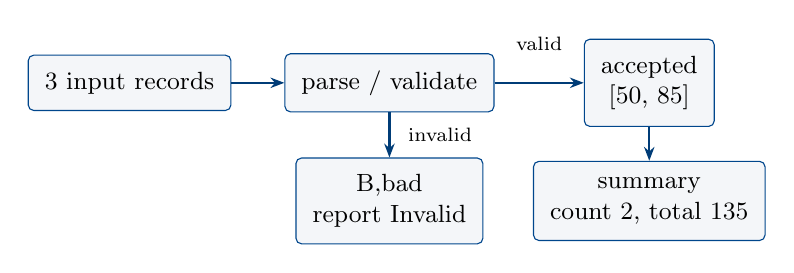
\begin{tikzpicture}
\node[draw=bkblue,rounded corners=2pt,fill=codebg,align=center,inner sep=6pt,font=\small] (read) at (0,0) {3 input records};
\node[draw=bkblue,rounded corners=2pt,fill=codebg,align=center,inner sep=6pt,font=\small] (parse) at (3.3,0) {parse / validate};
\node[draw=bkblue,rounded corners=2pt,fill=codebg,align=center,inner sep=6pt,font=\small] (store) at (6.6,0) {accepted\\[0pt] [50, 85]};
\node[draw=bkblue,rounded corners=2pt,fill=codebg,align=center,inner sep=6pt,font=\small] (reject) at (3.3,-1.5) {B,bad\\[0pt] report Invalid};
\node[draw=bkblue,rounded corners=2pt,fill=codebg,align=center,inner sep=6pt,font=\small] (sum) at (6.6,-1.5) {summary\\[0pt] count 2, total 135};
\draw[ref] (read) -- (parse);
\draw[ref] (parse) -- node[above=8pt,font=\scriptsize]{valid} (store);
\draw[ref] (parse) -- node[right=3pt,font=\scriptsize]{invalid} (reject);
\draw[ref] (store) -- (sum);
\end{tikzpicture}}

\column{0.3\textwidth}
\raggedright
\begin{contextbox}{Output}\begin{lstlisting}[style=code]
Invalid
2 135
\end{lstlisting}
\end{contextbox}
\end{columns}
\vspace{0.8em}
\small Attempted inputs and accepted records are different collections. Rejected data never contributes to a successful count or total. The shown numeric values are all within range.
\par\srcline{\href{../../weeks/week-12.html}{Course website: Week 12}. Complete programs accompany this deck.}

\end{frame}

\section{Team round 2: spot the errors}

\begin{frame}[fragile]{Spot the errors 1: Java (5 min)}
\begin{discussionbox}{Contract}\small Reject non-numeric and out-of-range marks. Count and sum only accepted records.\end{discussionbox}
\begin{columns}[T,onlytextwidth]
\column{0.48\textwidth}
\raggedright
\begin{lstlisting}[style=bad,language=Java,numbers=left,numberstyle=\tiny\color{codegray},firstnumber=1,numbersep=0.7em]
public class Broken {
    public static void main(String[] args) {
        String[] input={"A,50","B,bad","C,101"};
        int total=0,passed=0;
        for(String line:input) {
            try {
                int mark=Integer.parseInt(line.split(",")[1]);
                total+=mark;
                if(mark>50) passed++;
\end{lstlisting}

\column{0.48\textwidth}
\raggedright
\begin{lstlisting}[style=bad,language=Java,numbers=left,numberstyle=\tiny\color{codegray},firstnumber=10,numbersep=0.7em]
            } catch(NumberFormatException e) {
                System.out.println("Invalid");
            }
        }
        System.out.println("count,total,passed");
        System.out.println(input.length+","+total+","+passed);
    }
}
\end{lstlisting}

\end{columns}

\end{frame}

\begin{frame}[fragile]{Spot the errors 1: answers}
\begin{columns}[T,onlytextwidth]
\column{0.58\textwidth}
\raggedright
\begin{contextbox}{The repairs}\footnotesize\begin{itemize}[itemsep=0.45em]\item \textbf{L7:} After parsing, validate the domain range before updating any summary. Catch the validation failure too.\item \textbf{L9:} The pass boundary is inclusive: mark \textgreater{}= 50.\item \textbf{L15:} Count accepted records, not attempted input records.\end{itemize}\end{contextbox}
\column{0.38\textwidth}
\raggedright
\badlabel{Original program}\begin{lstlisting}[style=code]
Invalid
count,total,passed
3,151,1
\end{lstlisting}
\goodlabel{After the repairs}\begin{lstlisting}[style=code]
Invalid
Invalid
count,total,passed
1,50,1
\end{lstlisting}

\end{columns}
\par\srcline{\href{../../weeks/week-12.html}{Course website: Week 12}. Complete programs accompany this deck.}

\end{frame}

\begin{frame}[fragile]{Spot the errors 2: Python (5 min)}
\begin{discussionbox}{Contract}\small Reject malformed fields and invalid marks without stopping later records. Only valid marks contribute to the report.\end{discussionbox}
\begin{columns}[T,onlytextwidth]
\column{0.48\textwidth}
\raggedright
\begin{lstlisting}[style=bad,language=Py,numbers=left,numberstyle=\tiny\color{codegray},firstnumber=1,numbersep=0.7em]
lines=["A,50","broken","C,101"]
marks=[]
for line in lines:
    parts=line.split(",")
    try:
\end{lstlisting}

\column{0.48\textwidth}
\raggedright
\begin{lstlisting}[style=bad,language=Py,numbers=left,numberstyle=\tiny\color{codegray},firstnumber=6,numbersep=0.7em]
        marks.append(int(parts[1]))
    except ValueError:
        print("Invalid")
print("count,total,passed")
print(f"{len(lines)},{sum(marks)},{sum(m>50 for m in marks)}")
\end{lstlisting}

\end{columns}

\end{frame}

\begin{frame}[fragile]{Spot the errors 2: answers}
\begin{columns}[T,onlytextwidth]
\column{0.58\textwidth}
\raggedright
\begin{contextbox}{The repairs}\footnotesize\begin{itemize}[itemsep=0.45em]\item \textbf{L6:} Check the number of fields and a non-empty name before indexing.\item \textbf{L6:} Parse and validate 0..100 before appending.\item \textbf{L10:} Count successful records with len(marks).\item \textbf{L10:} Include exactly 50 in the pass count.\end{itemize}\end{contextbox}
\column{0.38\textwidth}
\raggedright
\badlabel{Original program}\begin{lstlisting}[style=code]
(no standard output)
IndexError: list index out of range
\end{lstlisting}
\goodlabel{After the repairs}\begin{lstlisting}[style=code]
Invalid
Invalid
count,total,passed
1,50,1
\end{lstlisting}

\end{columns}
\par\srcline{\href{../../weeks/week-12.html}{Course website: Week 12}. Complete programs accompany this deck.}

\end{frame}

\section{Team round 3: predict the output}

\begin{frame}[fragile]{Predict 1: References, collections and a boundary}
\begin{columns}[T,onlytextwidth]
\column{0.62\textwidth}
\raggedright
\begin{lstlisting}[style=code,language=Java]
import java.util.*;
public class Demo {
    static int count(List<Integer> xs) { int n=0; for(int x:xs) if(x>=50) n++; return n; }
    public static void main(String[] args) {
        List<Integer> a=new ArrayList<Integer>(Arrays.asList(49,50,85));
        List<Integer> b=a;
        List<Integer> c=new ArrayList<Integer>(a);
        b.remove(Integer.valueOf(49));
        c.set(0,0);
        System.out.println(a);
        System.out.println(c);
        System.out.println(count(a));
    }
}
\end{lstlisting}

\column{0.34\textwidth}
\raggedright
\begin{discussionbox}{Three minutes}\small Write every line in order. Explain the first state change, alias, dispatch decision or exception that controls the result. Then propose one change that alters the output.\end{discussionbox}
\end{columns}
\par\srcline{\href{../../weeks/week-12.html}{Course website: Week 12}. Complete programs accompany this deck.}

\end{frame}

\begin{frame}[fragile]{Predict 1: answer}
\begin{columns}[T,onlytextwidth]
\column{0.42\textwidth}
\raggedright
\begin{lstlisting}[style=code]
[50, 85]
[0, 50, 85]
2
\end{lstlisting}

\column{0.54\textwidth}
\raggedright
\begin{contextbox}{Why}\small Alias mutation affects a. The copied container c changes independently. count tests the inclusive boundary on the current a.\end{contextbox}
\end{columns}
\par\srcline{\href{../../weeks/week-12.html}{Course website: Week 12}. Complete programs accompany this deck.}

\end{frame}

\begin{frame}[fragile]{Predict 2: A record either enters the model or does not}
\begin{columns}[T,onlytextwidth]
\column{0.62\textwidth}
\raggedright
\begin{lstlisting}[style=code,language=Py]
def parse(text):
    name,raw=text.split(",")
    mark=int(raw)
    if not 0<=mark<=100: raise ValueError("range")
    return name,mark
records=[]
for line in ["A,50","B,bad","C,85"]:
    try: records.append(parse(line))
    except ValueError: print("Invalid")
print(len(records),sum(mark for name,mark in records))
print(sum(mark>=50 for name,mark in records))
\end{lstlisting}

\column{0.34\textwidth}
\raggedright
\begin{discussionbox}{Three minutes}\small Write every line in order. Explain the first state change, alias, dispatch decision or exception that controls the result. Then propose one change that alters the output.\end{discussionbox}
\end{columns}
\par\srcline{\href{../../weeks/week-12.html}{Course website: Week 12}. Complete programs accompany this deck.}

\end{frame}

\begin{frame}[fragile]{Predict 2: answer}
\begin{columns}[T,onlytextwidth]
\column{0.42\textwidth}
\raggedright
\begin{lstlisting}[style=code]
Invalid
2 135
2
\end{lstlisting}

\column{0.54\textwidth}
\raggedright
\begin{contextbox}{Why}\small The failed conversion prevents append. The two accepted tuples supply both the valid-record count and numeric summary.\end{contextbox}
\end{columns}
\par\srcline{\href{../../weeks/week-12.html}{Course website: Week 12}. Complete programs accompany this deck.}

\end{frame}

\section{Team round 4: write the code}

\begin{frame}[fragile]{Code it: specification}
\begin{discussionbox}{A complete marks pipeline}\small Read n then n records name,mark. Require exactly two fields, a non-empty name, and an integer mark in 0..100. Print Invalid immediately for each rejected record. Store accepted Student objects. Finish with count,total,passed and the summary of valid records.\end{discussionbox}
\begin{columns}[T,onlytextwidth]
\column{0.48\textwidth}
\raggedright
\neutrallabel{Example input}\begin{lstlisting}[style=code]
4
Linh,85
An,bad
Mai,50
Tea,101
\end{lstlisting}

\column{0.48\textwidth}
\raggedright
\neutrallabel{Expected output}\begin{lstlisting}[style=code]
Invalid
Invalid
count,total,passed
2,135,2
\end{lstlisting}

\end{columns}
\small Eight minutes. One Java team and one Python team at the keyboard. Other teams produce a boundary test and explain which wrong implementation it would expose.
\end{frame}

\begin{frame}[fragile]{Code it: Java solution (1/2)}
\begin{lstlisting}[style=code,language=Java,numbers=left,numberstyle=\tiny\color{codegray},firstnumber=1,numbersep=0.7em]
import java.util.*;
Scanner sc=new Scanner(System.in);
int n=Integer.parseInt(sc.nextLine());
List<Student> records=new ArrayList<Student>();
for(int i=0;i<n;i++) {
    String line=sc.nextLine();
    String[] parts=line.split(",",-1);
    try {
        if(parts.length!=2 || parts[0].isEmpty()) throw new IllegalArgumentException();
        int mark=Integer.parseInt(parts[1]);
        if(mark<0 || mark>100) throw new IllegalArgumentException();
        records.add(new Student(parts[0],mark));
    } catch(IllegalArgumentException e) { System.out.println("Invalid"); }
\end{lstlisting}
\par\srcline{\href{../../weeks/week-12.html}{Course website: Week 12}. Complete programs accompany this deck.}

\end{frame}

\begin{frame}[fragile]{Code it: Java solution (2/2)}
\begin{lstlisting}[style=code,language=Java,numbers=left,numberstyle=\tiny\color{codegray},firstnumber=14,numbersep=0.7em]
}
int total=0,passed=0;
for(Student student:records) { total+=student.mark(); if(student.passed()) passed++; }
System.out.println("count,total,passed");
System.out.println(records.size()+","+total+","+passed);
class Student {
    private final String name;
    private final int mark;
    Student(String name,int mark) { this.name=name; this.mark=mark; }
    int mark() { return mark; }
    boolean passed() { return mark>=50; }
}
\end{lstlisting}
\par\srcline{\href{../../weeks/week-12.html}{Course website: Week 12}. Complete programs accompany this deck.}

\end{frame}

\begin{frame}[fragile]{Code it: Python solution}
\begin{lstlisting}[style=code,language=Py,numbers=left,numberstyle=\tiny\color{codegray},firstnumber=1,numbersep=0.7em]
class Student:
    def __init__(self,name,mark): self.name,self.mark=name,mark
    def passed(self): return self.mark>=50
def parse(line):
    parts=line.split(",")
    if len(parts)!=2 or not parts[0]: raise ValueError("record")
    mark=int(parts[1])
    if not 0<=mark<=100: raise ValueError("range")
    return Student(parts[0],mark)
n=int(input())
records=[]
for _ in range(n):
    try: records.append(parse(input()))
    except ValueError: print("Invalid")
print("count,total,passed")
print(f"{len(records)},{sum(s.mark for s in records)},{sum(s.passed() for s in records)}")
\end{lstlisting}
\par\srcline{\href{../../weeks/week-12.html}{Course website: Week 12}. Complete programs accompany this deck.}

\end{frame}

\begin{frame}{Code it: the tests}
\footnotesize {\scriptsize A slash separates input lines; (blank) denotes an empty line.\par}\medskip \textbf{Test 1}\par \code{4 / Linh,85 / An,bad / Mai,50 / Tea,101}\par \textbf{Output:} \code{Invalid / Invalid / count,total,passed / 2,135,2}\par\medskip \textbf{Test 2}\par \code{0}\par \textbf{Output:} \code{count,total,passed / 0,0,0}\par\medskip \textbf{Test 3}\par \code{3 / A,0 / B,50 / C,100}\par \textbf{Output:} \code{count,total,passed / 3,150,2}\par\medskip \textbf{Test 4}\par \code{3 / missing / ,50 / a,b,c}\par \textbf{Output:} \code{Invalid / Invalid / Invalid / count,total,passed / 0,0,0}\par\medskip \keyline{Explain why each test is present, not only whether it passes.}
\end{frame}

\section{Wrapping up}

\begin{frame}{What you should now be able to explain}
\begin{itemize}[itemsep=0.6em]\item Explain a program through state changes and call contracts.\item Combine validation, models, collections and report formatting.\item Choose tests that distinguish a plausible wrong implementation.\item Treat functional transformations and streams as optional follow-on material.\end{itemize}\vfill\small Return to the matching week page for runnable examples and further practice. Bring one unresolved prediction or counterexample to the next class.\par\srcline{\href{../../weeks/week-12.html}{Course website: Week 12}. Complete programs accompany this deck.}

\end{frame}

\end{document}
